% what is a signal and what is a system?
%
% introduces:
% - signal
% - continuous-time and discrete-time signal
% - dependent and independent variable
% - system
%
\newthought{What is a signal and what is a system?} By
a \emph{\index{signal}{signal}}, we mean an information carrying
mathematical function. Any function that has a value as a function of
one or more variables is in essence a signal. By
a \emph{\index{system}{system}}, we denote a mathematical operation
that modifies a signal. A system consists of the precise mathematical
description of how a signal fed into a system is modified by the
system to produce an output signal.

The definitions of signals and a systems are merely abstract concepts,
which have gained acceptance in the engineering community. In the
context of mathematics, signals could also be called functions or
vectors. Systems would be called functions or operators. In computer
science, signals are often treated as arrays of numbers in the memory
of a computer and systems are algorithms and computer programs that
operate on these arrays.

\section{Signals}
\index{signal}

\begin{marginfigure}%
\begin{center}
\begin{tikzpicture}
\begin{axis}[width=\textwidth,
	xticklabels=\empty,
	yticklabels=\empty,		
	xmin=-1.5,xmax=6,
	axis x line=bottom,
	axis y line=left,
	xlabel={Independent variable $t$},
	xlabel style={below},
	ylabel={Dependent variable $x(t)$},
    xlabel style={ yshift = { 1em } },
    ylabel style={ yshift = { -2.2em } }
]
\addplot[draw=blue,domain=-1:7,samples=150] {(x>0)*exp(-x)};
\end{axis}
\end{tikzpicture}
\end{center}
\caption{Continuous-time signal.}
\label{fig:ctfig}
\end{marginfigure}

\begin{marginfigure}%
\begin{center}
\begin{tikzpicture}
\begin{axis}[width=\textwidth,
%	title={Discrete-time signal},
	xticklabels=\empty,
	yticklabels=\empty,	
	xmin=-1.5,xmax=6,
	axis x line=bottom,
	axis y line=left,
	xlabel={Independent variable $n$},
	xlabel style={below},
	ylabel={Dependent variable $x[n]$},
    xlabel style={ yshift = { 1em } },
    ylabel style={ yshift = { -2.2em } }
]
\addplot+[ycomb,domain=-1:5,samples=15] {(x>0)*exp(-x)};
\end{axis}
\end{tikzpicture}
\end{center}
\caption{Discrete-time signal.}
\label{fig:dtfig}
\end{marginfigure}


\newthought{A \index{signal}{signal}} is a mathematical function $x(t)$, which
describes the value of a \index{dependent variable} dependent variable
$x$, as a function of an \index{independent variable}independent
variable $t$. An independent variable ``sweeps'' through all possible
values. The dependent variable is the variable that changes as a
function of the independent variable and conveys information.

Here's an example. When describing electric potential as a function of
time $V(t)$, time $t$ is the independent variable and the electric
potential $V(t)$ as a function of time is the dependent variable. Time
by itself does not convey information, but electric potential as a
function of time does.

Physical ``real world'' signals are modeled as continuous-time
signals. Examples include, amongst countless others:
\begin{itemize}
 \setlength\itemsep{0.25em}        
\item temperature,
\item density,
\item pressure as a function of time and space (sound, seismic waves),
\item electric field as a function of time and position
  (electromagnetic waves), or
\item electrical current in a circuit.
\end{itemize}
Physics relies on differential calculus, with integration and
differentiation as elementary operators. As we will later see,
differential calculus can be studied through methods of signal
processing. Especially the spectral techniques and the Fourier
transform are useful tools that can be applied in differential
calculus.

This course will focus primarily on one-dimensional signals. These
signals are complex valued functions $x(t) \in \mathbb{C}$ of a real
valued argument $t\in \mathbb{R}$. This will naturally also cover the
special case, where the signal is real valued
$x(t) \in \mathbb{R} \subset
\mathbb{C}$. 

By convention, we will refer to the independent variable of a signal
as time, even though this variable doesn't necessarily have to
indicate time. It can represent anything. For example, the independent
variable can just as well be e.g., distance.

Signals can be continuous or discrete. Following a commonly adopted
practice, we will use round brackets for continuous-time signals
(e.g., $x(t)$) and square brackets for discrete-time signals (e.g.,
$x[n]$). 

In the case of discrete-time signals, the sample index
$n \in \mathbb{Z}$ is unitless. A discrete-time signal is merely a
sequence of numbers. The only way to associate meaning to this
sequence of numbers is the a priori knowledge of how the signal was
discretized. This allows us to e.g., map the $n$th sample to a real
valued time.

An example of a continuous-time and a discrete-time signal is shown in
Figures \ref{fig:ctfig} and \ref{fig:dtfig}. When plotting signals
graphically, it is customary (but not mandatory) to use the horizontal
axis for the independent variable, and the dependent variable on the
vertical axis.

To summarize, the two main types of signals that this course deals
with are one-dimensional continuous-time $x(t)$ and one-dimensional
discrete-time signals $x[n]$. Continuous-time signals are mappings
from the real axis (time) to the set of complex numbers:
\begin{equation}
\boxed{
x: \mathbb{R} \rightarrow \mathbb{C}
}
\end{equation}
Discrete-time signals are mappings from the set of integers to the set of complex numbers:
\begin{equation}
\boxed{
x: \mathbb{Z} \rightarrow \mathbb{C}
}
\end{equation}
Signal processing of higher dimensional signals are essentially functions of the form
\begin{equation}
x: \mathbb{R}^N \rightarrow \mathbb{C}
\end{equation}
or in the case of discrete-time:
\begin{equation}
x: \mathbb{Z}^N \rightarrow \mathbb{C}
\end{equation}

\newthought{The first experimental detection of gravitational waves}
using the Laser Inteferometer Gravitational-Wave Observatory (LIGO) is
shown in Figure \ref{fig:ligo_meas}. This signal is an example of a
one-dimensional signal. The signal is thought to be caused by two
black holes with masses around 30 solar masses merging together, 1.3
billion light-years from Earth. The independent variable on the x-axis
is time, and the dependent variable is strain (stretching) of space
that occurs due to a gravitational wave passing through the
instrument. This is measured by comparing the relative lengths of two
4 km long laser interferometer arms. 

\begin{figure}
\begin{center}
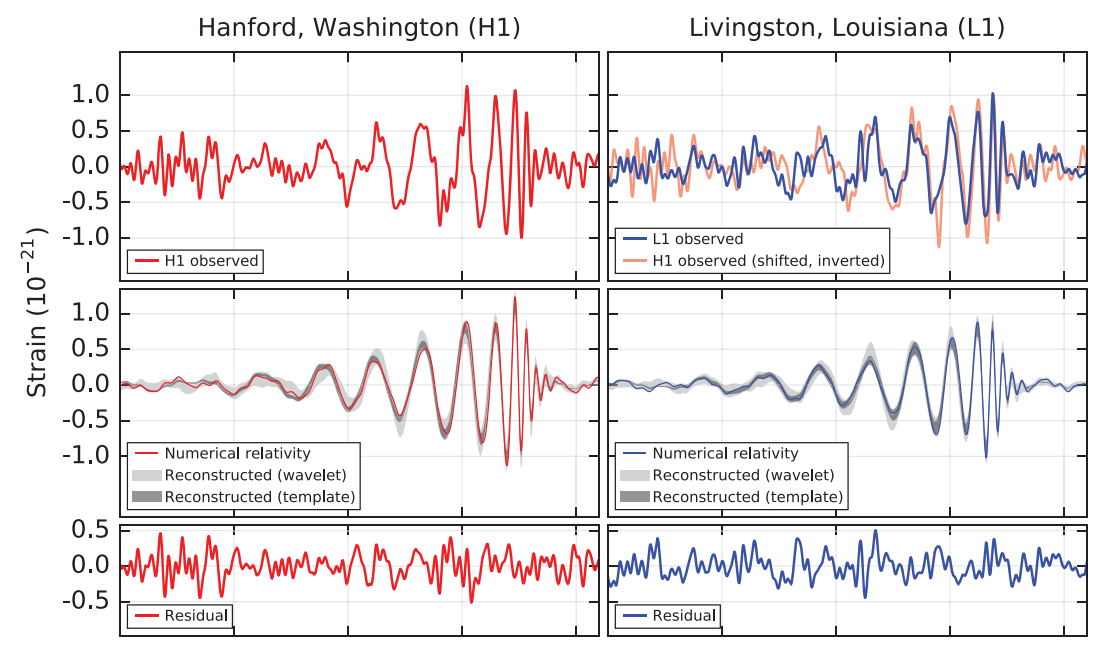
\includegraphics[width=\textwidth]{ch04/figures/dc_fg.png}
\end{center}
\caption{Two independent one dimensional signals measured by LIGO depicting strain. This is stretching of space due to a gravitational wave passing through two geographically separated laser interferometer observatories. One in Hanford, WA (left), and one in Livingston, LA (right). The figure is from: B. P. Abbott et al. (LIGO Scientific Collaboration
and Virgo Collaboration) Phys. Rev. Lett. 116, 061102 – Published 11
February 2016.}
\label{fig:ligo_meas}
\end{figure}

\newthought{Signals can be of arbitrary dimension}. For example, an image is a 2d
signal, where the dependent variable is intensity $I(x,y)$ measured as
a function of two independent spatial variables $x$ and $y$ that
indicate distance from origin along two orthogonal axes.  An example
of a discrete-time two-dimensional signal is shown in Figure
\ref{fig:bh_example}. It represents an image of the emission from hot gas in the
event horizon of a black hole around the M87 galaxy. The image is
obtained using a technique called very long baseline interferometry,
which utilizes measurements from radio telescopes around the
world. These measurements are combined together to simulate a large
telescope with the resolution equivalent to a telescope approximately
the size of Earth.\footnote{The Fourier transform, which is one of the
central themes in this course, is a key part of the mathematics of
very long baseline interferometric imaging.}

Even higher dimensional signals can be used. Consider for example a
video. It is a signal that contains the intensity of an image as a
function of time. You can think of a moving picture (movie) as a three
dimensional signal: $I(x,y,t)$, where the intensity of the image is a
function of two dimensional position as well as time.

While we will focus primarily on one dimensional signals in order to
keep things simple, many of the concepts we discuss can be generalized
to multiple dimensions. Two dimensional signal processing is called
image processing, and it shares many of the same basic concepts with
one dimensional signal processing. I will try to also occasionally
give examples of signal processing with higher dimensional signals.


%\begin{figure}
%\begin{center}
%\includegraphics[width=\textwidth]{ch01/2dsig.png}
%\end{center}
%\label{fig:2dexim}
%\caption{An example of a 2d signal: 32-cm wavelength opposite
%  circularly polarized inverse synthetic aperture radar map of the
%  Moon, obtained using the EISCAT radar in Troms\o{}. Image intensity
%  represents backscattered power from the surface of the Moon.}
%\end{figure}

\begin{figure}
\begin{center}
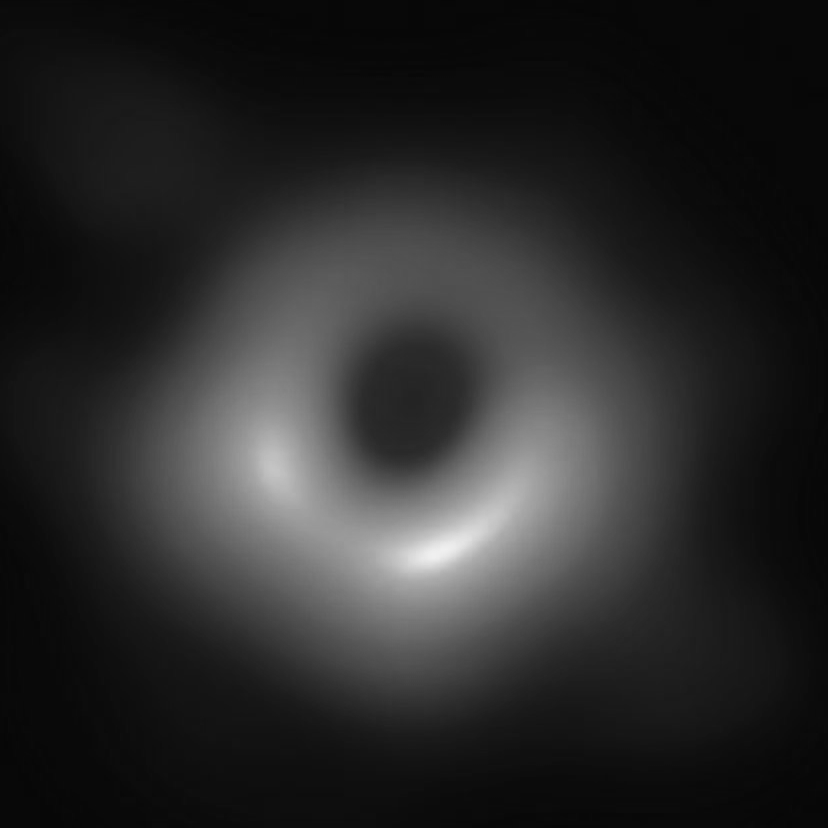
\includegraphics[width=0.68\textwidth]{ch04/figures/bhi.png}
\end{center}
\caption{An example of a 2d signal: A Very Long Baseline Interferometric radio image of
the black hole at the center of galaxy M87. The intensity depicts what
is thought to be hot gas outside the event horizon of the black hole.
Credit: Event Horizon Telescope collaboration et al. 2019.}
\label{fig:bh_example}
\end{figure}

\newthought{Digital signals}
in a computer are also quantized. This means that there is only a
finite number of possible values for the dependent value of a
signal. This type of a signal is called
a \emph{\index{quantized}{quantized}} signal. We will not discuss
quantization in this course.


\section{Systems}
%\newcommand{\sign}{\text{sign}}

\newthought{A signal processing \index{system}{system}} can be represented
graphically as a block diagram, which describes signals going into a
system, and signals going out of a system. An example is shown in
Figure \ref{simple_sps}

\begin{figure}
\tikzstyle{int}=[draw]
%\tikzstyle{init} = [pin edge={to-,thin,black}]
\tikzstyle{init} = []
% [pin edge={to-,thin,black}]

\begin{center}
  \begin{tikzpicture}[node distance=4cm,auto,line width=0.1mm,>=triangle 45]
    \node [int] (a) {System $\spop$};
    \node (b) [left of=a,node distance=4cm, coordinate] {a};
    %\node [int, pin={[init]above:$p_0$}] (c) [right of=a] {$\frac{1}{s}$};
    \node [coordinate] (end) [right of=a, node distance=4cm]{};
    \path[->] (b) edge node {signal in $x(t)$} (a);
    %\path[->] (a) edge node {$v$} (c);
    \draw[->] (a) edge node {signal out $y(t)$} (end) ;
\end{tikzpicture}
\end{center}
\label{simple_sps}
\caption{A simple signal processing system block diagram.}
\end{figure}
A graphical representation is useful for understanding a signal
processing system, especially if it is a complicated one, which
includes many systems and signals.

The following block diagram is a real-world example of the block diagram of the EISCAT Svalbard radar transmitter subsystem. 
\begin{figure}
\begin{center}
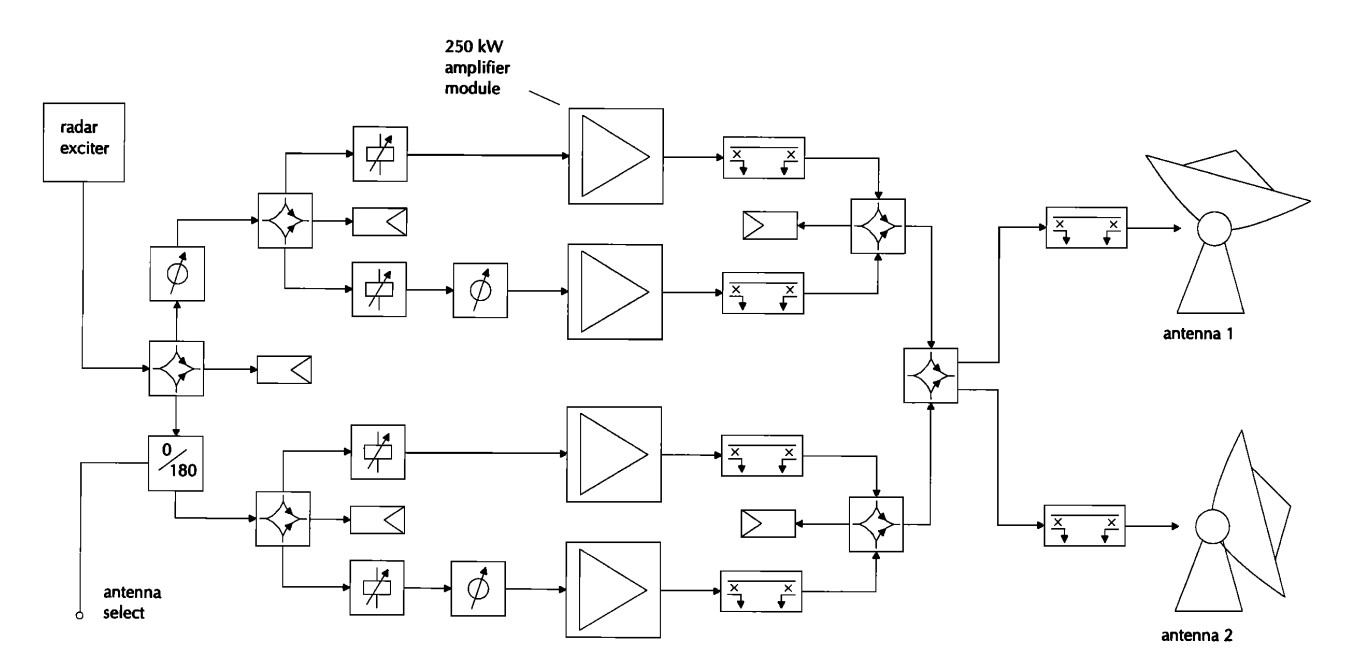
\includegraphics[width=\textwidth]{ch04/figures/wannberg97.jpg}
\end{center}
\caption{An example of a more complicated block diagram. From: Wannberg et.al., 1997.}
\label{fig:esr}
\end{figure}

The mathematical description of a system (what goes on in the box) is
a general transformation of a signal. The mathematical notation for a
continuous-time system in general is\footnote{Here $\spop$ is a
  mathematical description of how the input signal is modified by the
  signal processing system. This is also called an
  \index{operator}{operator}}:
\begin{equation}
\boxed{
y(t) = \spop[x(t)]
}
\end{equation}
and for discrete-time system:
\begin{equation}
\boxed{
y[n] = \spopb\{x[n]\}
}
\end{equation}
An example of a system could be a function that delays the input
signal by a delay $\tau$ :
\begin{equation}
y(t) = x(t-\tau).
\end{equation}
Another example is a linear amplifier, which multiplies the amplitude
of the signal with a constant $\alpha \in \mathbb{C}$:
\begin{equation}
y(t) = \alpha x(t).
\end{equation}
You will often encounter both of these types of systems.

\newthought{For example, we can use these two basic systems to make a simplified
model of a radar}. Imagine that you have a radar. This radar sends out
a waveform that is described by a waveform $x(t)$. Let's say that the
time it takes an electromagnetic wave to travel from the radar
transmitter to a point-like radar target and back is $\tau$
seconds. The received radar echo will be a delayed version of the
transmitted signal, which is delayed by $\tau$. In addition to this,
the signal will be scaled, as a radar echo is typically much weaker
than the transmitted signal.

Therefore, a very simple system that describes a radar echo is the
following:
\begin{equation}
y(t) = \alpha x(t-\tau)
\end{equation}
where $y(t)$ is the received radar echo signal.

We can further expand this concept to write the equation that
describes a radar echo for a situation where there can be a continuous
radar echo at time delays between $0$ and $T$:
\begin{equation}
y(t) = \int_0^T \alpha(\tau) x(t-\tau) d\tau.
\end{equation}
In this case, $\alpha(\tau)$ describes the radar echo amplitude as a
function of propagation delay. This type of an equation is called
a \emph{\index{convolution}convolution} equation. You will encounter
this type of an equation very often in signal processing, and find
that the Fourier transform is a very useful tool when dealing with
convolution equations.

\newthought{Differential operators can also be seen as
systems}. Consider the first time-derivative of the continuous-time signal $x(t)$:
\begin{equation}
y(t) = \frac{d}{d t}x(t).
\end{equation}
The system definition is the time derivative operator $\frac{d}{dt}$.

\newthought{Systems are classified based on their mathematical properties}. The
most important two are: \emph{\index{linearity}{linearity}} and \emph{\index{time-invariance}{time-invariance}}. A
system which is both linear and time-invariant is called 
\index{linear time-invariant}{linear time-invariant} 
(LTI)\index{LTI}. Such systems have beneficial mathematical properties
that make analysis and design of such systems very
straightforward. We'll later on prove that LTI systems are fully
characterized by something known as a impulse response. This is an
important concept in signal processing.

\section{Linear system}
\index{Linear system}

\begin{marginfigure}[-3cm]
\tikzstyle{int}=[draw, minimum size=2em]
\tikzstyle{init} = [pin edge={to-,thin,black}]

\begin{center}
% Definition of blocks:
\tikzset{%
  block/.style    = {draw, thick, rectangle, minimum height = 3em,
    minimum width = 3em},
  sum/.style      = {draw, circle, node distance = 2cm}, % Adder
  input/.style    = {coordinate}, % Input
  output/.style   = {coordinate} % Output
}
% Defining string as labels of certain blocks.
\newcommand{\suma}{\Large$+$}
\newcommand{\inte}{$\displaystyle \int$}
\newcommand{\derv}{\huge$\frac{d}{dt}$}
\newcommand{\mula}{\Large$\cross$}

\begin{tikzpicture}[auto, line width=0.1mm, node distance=2cm, >=triangle 45]
% make an op block
\draw 
   node at (0,0) [block, name=op0] {$\spop$};
% make a sum block
\draw 
   node at (-1.5,0) [sum, name=suma2] {\suma};
% output node
\draw 
   node at (1.5,0) [name=out0] {$y_1(t)$};

% input node 1
\draw 
   node at (-3,1.5) [name=in0] {$x_1(t)$};

% input node 2
\draw 
   node at (-3,-1.5) [name=in1] {$x_2(t)$};

% make a mult block
\draw 
   node at (-1.5,1.5) [sum, name=mul0] {\mula};
% make a mult block
\draw 
   node at (-1.5,-1.5) [sum, name=mul1] {\mula};

% output node
\draw 
   node at (0,1.5) [name=c0] {$c_2$};

% output node
\draw 
   node at (0,-1.5) [name=c1] {$c_1$};

% join
\draw[->](suma2) -- node {}(op0);
\draw[->](mul0) -- node {}(suma2);
\draw[->](mul1) -- node {}(suma2);
\draw[->](op0) -- node {}(out0);
\draw[->](in0) -- node {}(mul0);
\draw[->](in1) -- node {}(mul1);
\draw[->](c0) -- node {}(mul0);
\draw[->](c1) -- node {}(mul1);
\end{tikzpicture}

\vspace{1em}
\begin{tikzpicture}[auto, line width=0.1mm, node distance=2cm, >=triangle 45]
% make an op block
\draw 
   node at (-1.5,1.5) [block, name=op0] {$\spop$};

\draw 
   node at (-1.5,-1.5) [block, name=op1] {$\spop$};

% make a sum block
\draw 
   node at (0,0) [sum, name=suma2] {\suma};

% make a mult block
\draw 
   node at (0,1.5) [sum, name=mul0] {\mula};

% make a mult block
\draw 
   node at (0,-1.5) [sum, name=mul1] {\mula};

% output node
\draw 
   node at (1.5,0) [name=out0] {$y_2(t)$};

% output node
\draw 
   node at (1.5,1.5) [name=c0] {$c_2$};

% output node
\draw 
   node at (1.5,-1.5) [name=c1] {$c_1$};

% input node 1
\draw 
   node at (-3,1.5) [name=in0] {$x_1(t)$};
% input node 2
\draw 
   node at (-3,-1.5) [name=in1] {$x_2(t)$};

% join
\draw[->](suma2) -- node {}(out0);

\draw[->](in0) -- node {}(op0);
\draw[->](in1) -- node {}(op1);

\draw[->](op0) -- node {}(mul0);
\draw[->](op1) -- node {}(mul1);
\draw[->](mul0) -- node {}(suma2);
\draw[->](mul1) -- node {}(suma2);
\draw[->](c0) -- node {}(mul0);
\draw[->](c1) -- node {}(mul1);

\end{tikzpicture}
\end{center}
\label{fig:linearity_block}
\caption{In order for the system specified by $\spop$ to be linear,
  $y_1(t) = y_2(t)$ must be satisfied.}
\end{marginfigure}

A system is linear, if a linear combination of inputs fed into the
system yields the same as the linear combination of outputs:
\begin{equation}
\boxed{
c_1 \spop[x_1(t)] + c_2 \spop[ x_2(t) ] = \spop[c_1 x_1(t) + c_2 x_2(t)]}
\end{equation}
for arbitrary constants $c_1 \in \mathbb{C}$ and $c_2 \in \mathbb{C}$
and arbitrary input signals $x_1(t)$ and $x_2(t)$. This property is
highly useful, and appears throughout signal processing.

\newthought{An example of a linear system} is a system that scales the
input signal by a constant factor $\alpha$:
\begin{equation}
  y(t) = \alpha x(t).
\end{equation}
If $|\alpha| >1$, the signal is amplified. This type of a system would
typically be called an amplifier. If $0<|\alpha|<1$, the system would
be called an attenuator, as the output signal amplitude would be
attenuated.

It is quite easy to determine that the test for linearity is passed for this system:
\begin{equation}
c_1 [\alpha x_1(t)] + c_2 [\alpha x_2(t)] = \alpha [c_1 x_1(t) + c_2 x_2(t)].
\end{equation}

\newthought{An example of a non-linear system} is the following system, which obtains the absolute value of $x(t)$:
\begin{equation}
y(t) = |x(t)|
\end{equation}
It is quite clear that this does not pass the test for linearity:
\begin{equation}
c_1 |x_1(t)| + c_2 |x_2(t)| \ne |c_1 x_1(t) + c_2 x_2(t)|.
\end{equation}
for all possible values $c_1$, $c_2$, $x_1(t)$, and $x_2(t)$.
\begin{marginfigure}
\tikzstyle{int}=[draw, minimum size=2em]
\tikzstyle{init} = [pin edge={to-,thin,black}]

\begin{center}

% Definition of blocks:
\tikzset{%
  block/.style    = {draw, thick, rectangle, minimum height = 3em,
    minimum width = 3em},
  sum/.style      = {draw, circle, node distance = 2cm}, % Adder
  input/.style    = {coordinate}, % Input
  output/.style   = {coordinate} % Output
}
% Defining string as labels of certain blocks.
\newcommand{\suma}{\Large$+$}
\newcommand{\inte}{$\displaystyle \int$}
\newcommand{\derv}{\huge$\frac{d}{dt}$}
\newcommand{\mula}{\Large$\cross$}

\begin{tikzpicture}[auto, line width=0.1mm, node distance=2cm, >=triangle 45]


% make an op block
\draw  
node at (-1.0,3.0) [name=in0] {$x(t)$};

% make an op block
\draw  
node at (-1.0,1.5) [block, name=op0] {$\spop$};

\draw  
node at (-1.0,0) [block, name=delay0] {Delay};

% output node
\draw 
 node at (-1.0,-1.5) [name=out0] {$y_2(t)$};


% make an op block
\draw  
node at (1.0,3.0) [name=in1] {$x(t)$};

% make an op block
\draw  
node at (1.0,0.0) [block, name=op1] {$\spop$};

\draw  
node at (1.0,1.5) [block, name=delay1] {Delay};

% output node
\draw 
 node at (1.0,-1.5) [name=out1] {$y_1(t)$};



% join
\draw[->](in0) -- node {}(op0);
\draw[->](op0) -- node {}(delay0);
\draw[->](delay0) -- node {}(out0);


% join
\draw[->](in1) -- node {}(delay1);
\draw[->](delay1) -- node {}(op1);
\draw[->](op1) -- node {}(out1);


\end{tikzpicture}


\end{center}
\caption{In order for the system specified by $\spop$ to be time-invariant, $y_1(t) = y_2(t)$ must be satisfied. \label{fig:time_inv_block}}
\end{marginfigure}


\section{Time-invariant system}
\index{Time-invariant}

Let us first define a delay system $\mathcal{D}\{x(t)\} = x(t-\tau)$. Let us assume that the output of a system is $y(t) = \spop[x(t)]$. This system is time-invariant if:
\begin{equation}
\boxed{
\mathcal{T}\{\mathcal{D}\{x(t)\}\} = \mathcal{D}\{\mathcal{T}\{x(t)\}\}
}
\end{equation}
In other words, it does not matter if the signal is delayed before or
after the system $\mathcal{T}\{\cdot\}$.

Time-invariance can be formally tested by using this equation and
comparing the output of a system for a time-shifted input $y_1(t) =
\spop[\mathcal{D}\{x(t)\}]$ to a time-shifted output signal $y_{2}(t)
= \mathcal{D}\{\mathcal{T}\{x(t)\}\}$:
\begin{align}
y(t) &= \spop[x(t)] \\
y_1(t) &= \spop[\mathcal{D}\{x(t)\}] = \spop[x(t-\tau)]\\
y_2(t) &= \mathcal{D}\{\mathcal{T}\{x(t)\}\} = y(t-\tau).
\end{align}
If $y_1(t) = y_2(t)$, the system is time-invariant. Otherwise not. The
test for time-invariance is illustrated as a block diagram in Figure
\ref{fig:time_inv_block}.

\newthought{An example of a time-invariant system} is the system that
returns the absolute value of the input signal $y(t)=|x(t)|$. We can
see this by evaluating:
\begin{align}
y(t) &= |x(t)|\\
y_1(t) &= |x(t-\tau)|\\
y_2(t) &= y(t-\tau) = |x(t-\tau)|
\end{align}
Time-invariance holds, because it is easy to see that
$y_1(t)=y_2(t)$. It doesn't matter if a time-delay is applied to the
signal before or after obtaining the absolute value of the input signal.

\newthought{An example of a case that is not time-invariant} is $y(t)
= t + x(t)$. We can immediately see that the system directly depends
on $t$, not only through the input. The formal test also shows that
time-invariance is not met:
\begin{align}
y(t) &= t + x(t)\\
y_1(t) &= t + x(t-\tau)\\
y_2(t) &= y(t-\tau) = t - \tau + x(t-\tau)
\end{align}
In this case $y_1(t) \ne y_2(t)$.


\section{Example: Overdriven amplifier}
\label{dist_effect}

\begin{marginfigure}
\begin{tikzpicture}
	\begin{axis}[
		xmin=-3, xmax=3,
		height=7cm,
		width=7cm,
		axis x line=center,
		axis y line=center,
                ylabel=$y(t)$,
		xlabel=$x(t)$
	]
		
	\addplot[mark=none,color=blue] {2*x};
	\addlegendentry{$y(t)$}

	\addplot[mark=none,color=red] coordinates {
		(-100,-3)
		(-1.5,-3)
		(1.5,3)
		(100,3)
	};
	\addlegendentry{$y_d(t)$}
	\end{axis}
\end{tikzpicture}
\caption{The system function of a linear amplifier $y(t)$ and a clipping amplifier system $y_d(t)$.}
\end{marginfigure}

A simple model of a distorted guitar amplifier system would be the
following clipping amplifier system, which is specified as follows:
\begin{equation}
y_d(t) = \left\{
  \begin{array}{rcr}
    -\beta & \mathrm{when} & \alpha x(t)<-\beta \\
    \alpha x(t) & \mathrm{when} & |\alpha x(t)| \le \beta \\
    \beta & \mathrm{when} & \alpha x(t)>\beta 
\end{array}
\right.
\label{clipamp}
\end{equation}
This is a very approximative model of an overdriven guitar
amplifier. This type of a system is often encountered in guitar music
from 50s and onwards. I'm sure that once you later implement this in
practice, you'll recognize the sound that this system makes.

What does this system do? It amplifies the signal, but only up to a
certain point. Beyond a certain absolute value of the input, the
output maintains a constant positive or negative value.  This type of
a behavior is also sometimes called clipping, and the effect is
also sometimes called distortion, as the input signal amplitude is not
linearly scaled, but it is rather distorted.

\begin{marginfigure}
  \begin{center}
    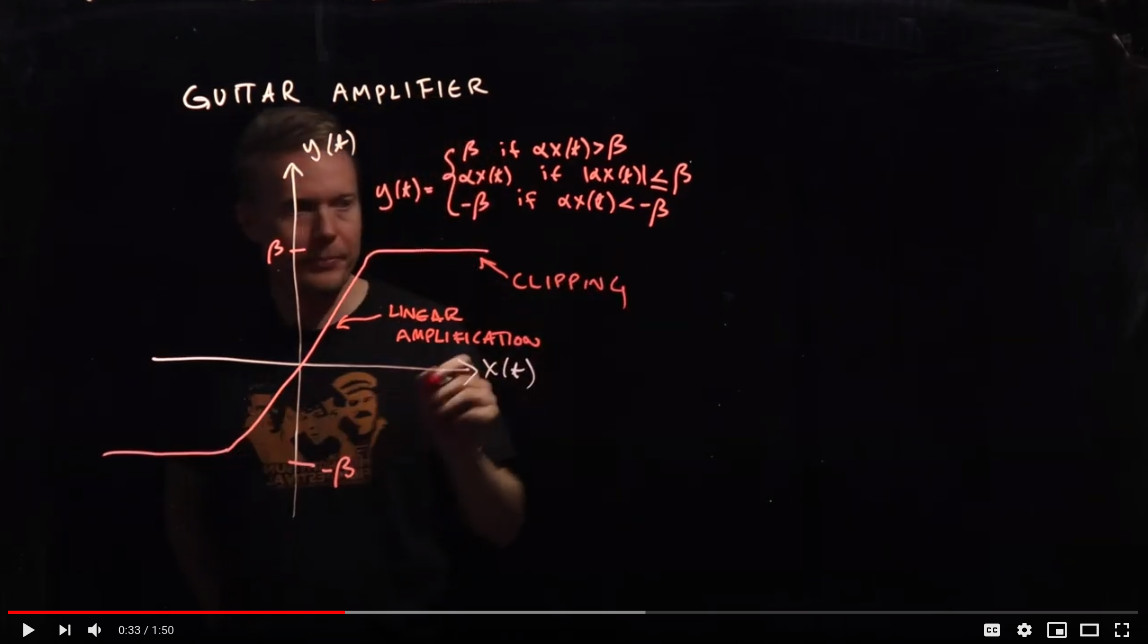
\includegraphics[width=\textwidth]{ch04/figures/ampvid.jpg}
  \end{center}
  \caption{A video discussing an overdriven guitar amplifier can be found here: \url{https://youtu.be/I30Mn_-yYF8}.}
\end{marginfigure}
Many real world amplifier systems have this type saturation
behaviour. What this often means in practice is that the system is
linear when the input absolute amplitude is less than some critical
value, but beyond this, linearity no longer holds.

The Figure below illustrates what $y_d(t)$ would look like as a
function of $x(t)$. It is compared with a normal amplifier system
$y(t)=\alpha x(t)$, which does not clip.

\if 0
\begin{center}
\includegraphics[width=0.68\textwidth]{ch01_guitar_amp/clipamp.png}
\end{center}
\fi
